\section{Static Load Balancing}
\label{sec:static-load-balancing}

To motivate the need for load balancing we show how limiting the cache size
saves memory and sacrifices neglible performance. This type of analysis will
help inform our load balancing policies for when we switch to a distributed
key-value store backend to store segment coordinates.  We need to know when and
how to partition the keyspace: a smaller cache hurts performance because
key-value pairs need to be retrieved from other nodes while a larger cache has
higher memory usage. 

% techinical details
On each cache node, ParSplice uses an infinitely large cache to store segment
coordinates. We limit the size of the cache using an LRU eviction policy, where
the penalty for a cache miss is retrieving the data from the persistent
database.  We evict keys (if necessary) at every operation instead of when
segments complete because the cache fills up too quickly otherwise and it
reduces the overhead of key eviction.

% results: cache size trade-offs
\subsubsection*{Results}
The results for different cache sizes for a growth rate of 100K over a 2.5 hour
run is shown in the left two plots of Figure~\ref{fig:methodology-tradeoff}.
``Baseline" is the performance of unmodified ParSplice  measured in trajectory
duration (\(y\)-axis) and utilization is measured with memory footprint (\(y2\)
axis) of just the cache.  ``Static Load Balancing Policies" shares the
\(y\)-axis and shows the trade-off for different cache sizes. The error bars
are the standard deviation of 3 runs. 

% results: raw numbers
Although the keyspace grows to 150K, a 100K key cache achieves 99\% of the
peformance. Decreasing the cache degrades performance and predictability.  Not
suprisingly, the memory usage all decreases with the cache size and although we
only save 0.4GB, larger and more complicated runs use up to 4GB, which is 3\%
of the 128GB on each node.  While this result is not unexpected, it nonetheless
achieves our goal of showing the benefits of load balancing keys across nodes
and that smaller caches on each node are an effective way to save memory
without completely sacrificing performance.

\begin{figure*}[tbh]
  \noindent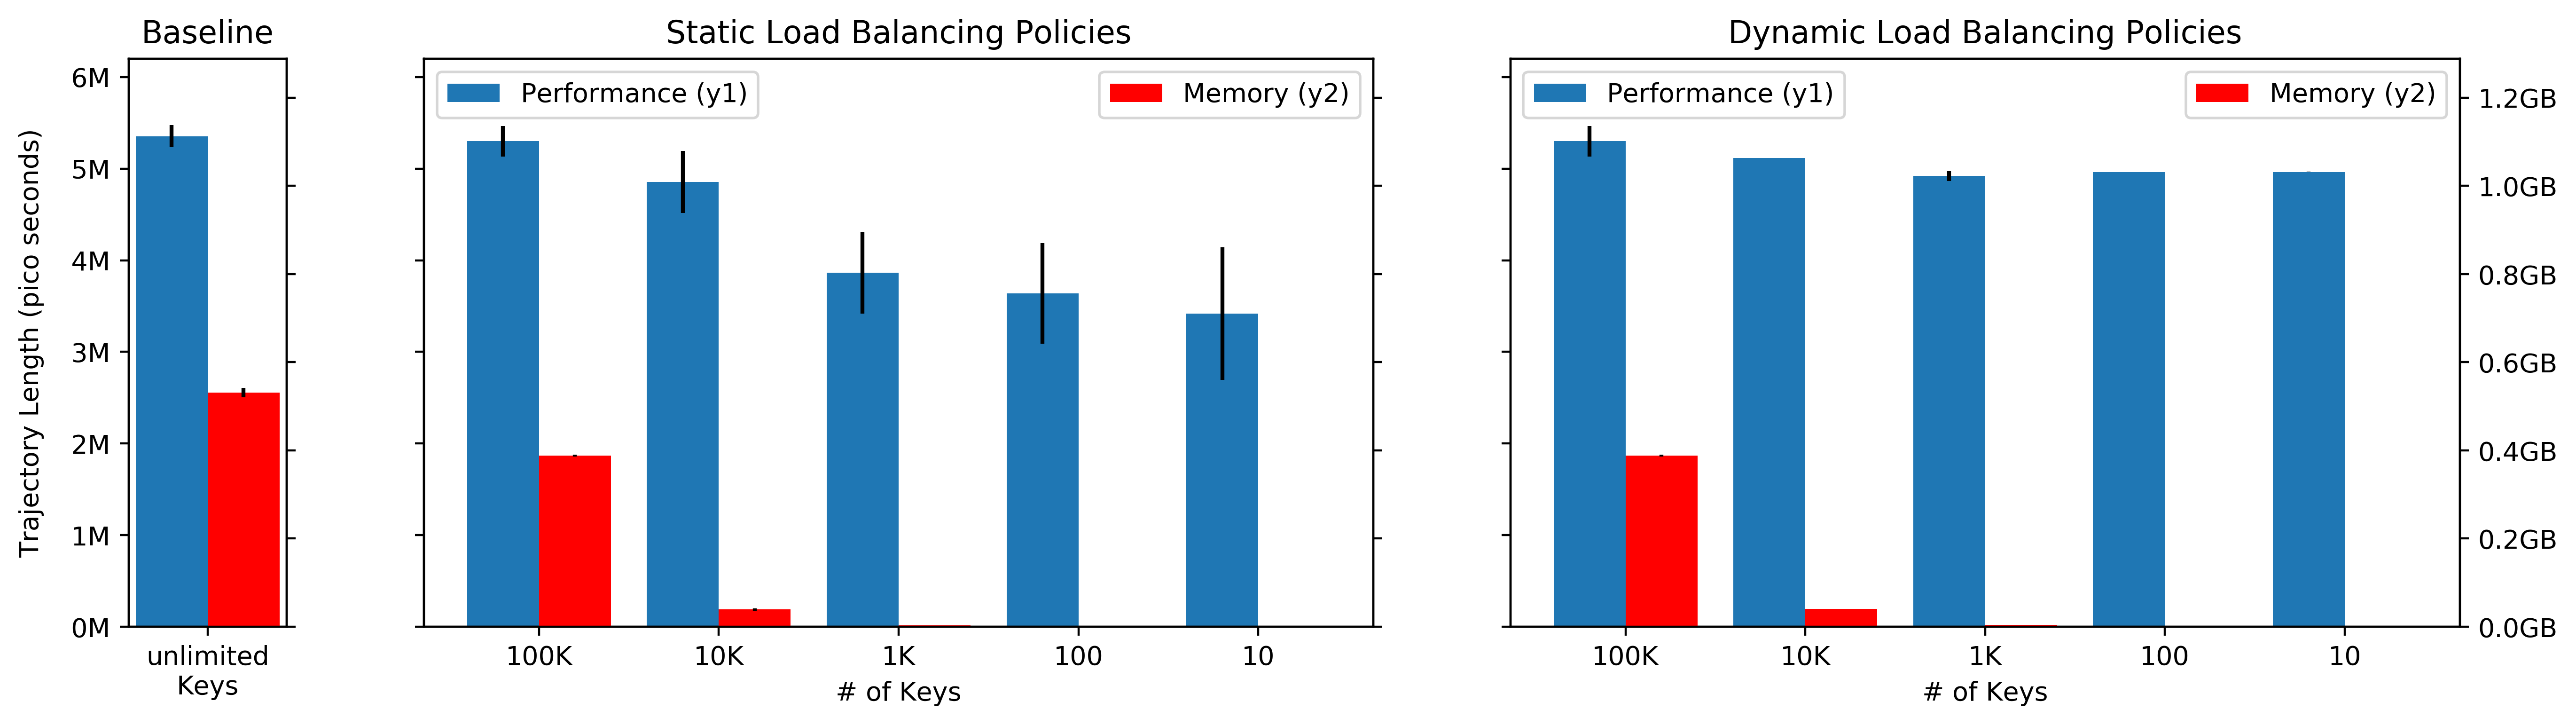
\includegraphics[width=1\textwidth]{figures/methodology-tradeoff.png}\\
  \caption{The performance and resource utilzation trade-off for different
  cache sizes, which are enumerated along the \(x\)-axes. ``Baseline" is
  ParSplice unmodified, ``Static Load Balancing Policies" limits the size of the
  cache to demonstrate the benefits of smaller keyspaces on cache nodes
  (Section~\S\ref{sec:static-load-balancing}), and ``Dynamic Load Balancing
  Policies" switches to a smaller cache after absorbing the initial burstiness of
  the workload
  (Section~\S\ref{sec:the-need-for-dynamic-load-balancing-policies}).
  \label{fig:methodology-tradeoff}}
\end{figure*}

\section{The Need for Dynamic Load Balancing Policies}
\label{sec:the-need-for-dynamic-load-balancing-policies}

% why is the performance lower for smaller caches?
Despite the memory savings, our results suggest that dynamic load balancing
policies could save even more memory.  The left two plots in
Figure~\ref{fig:methodology-tradeoff} show that a 100K key cache is sufficient
as a static policy but the top graph in Figure~\ref{fig:futurework-regimes}
indicates that the cache size could be much smaller. That graph shows that the
beginning of the run is characterized by many reads to a small set of keys and
the end sees much lower reads per second to a larger keyspace. Specifically, it
shows only about 100 keys as active in the latter half of the run, so a smaller
cache should indeed suffice. 

After analyzing traces, we see that the 100 key cache is insufficient because
LevelDB cannot service the read-write traffic. By limiting the size of the
cache, some reads must traverse up the ParSplice cache hierarchy to the
persistent database.  According to Figure~\ref{fig:futurework-regimes}, the
read requests arrive at 750 reads per second in addition to the writes that
land in each tier (about 300 puts/second, some redundant). This traffic
triggers a LevelDB compaction and reads block and eventually pile up, resulting
in very slow progress. Traces verify this hypothesis and show reads getting
backed up as the read/write ratio explodes. To recap, small caches incurr too
much load on persistent database  at the beginning of the run but smaller caches should
suffice after the initial read flash crowd passes because the keyspace is far
less active. This suggests a two-part load balancing policy.

% what is mantle
To explore dynamic load balancing policies ({\it i.e.} policies that change
during the run), we use the Mantle approach.  Mantle is a framework buit on the
Ceph file system that lets admnistrators control file system metadata load
balancing policies. The basic premise is that load balancing policies can be
expressed with a simple API consisting of ``when", ``where", and ``how much".
The succinctness of the API lets users inject muitiple, dynamic policies.

% Why is this a good idea
Although ParSplice does not use a distibuted file system, its workload is very
similiar because the minima key-value store responds to small and frequent
requests, which results in hot spots and flash crowds.  Distributed file
systems solve similiar issues: since data IO does not scale like metadata
IO~\cite{roselli:atec2000-FS-workloads}, finding optimal ways to measure,
migrate, and partition metadata load is a relatively new field, but has been
shown to lead to large performance increases and more scalable file
systems~\cite{zheng:pdsw2014-batchfs, zheng:pdsw2015-deltafs, grider:pdsw2015-marfs,
ren:sc2014-indexfs, patil:fast2011-giga+, brandt:msst2003-lh}.  Both workloads
also have data locality so the storage should have mechanisms for leveraging
requests with similar semantic meaning.  Previous work quantified the speedups
achieved with Mantle and formalized balancers that were good for file systems.

% why is it awesome.
%Mantle controls how to distribute or concentrate file system metadata and helps
%users quantify the effects of load balancing.  The paper identified effective
%file system load balancing policies and tested them under metadata-intensive
%workloads. The Greedy Spill balancer, which was based
%on~\cite{patil:fast2011-giga+}, sheds half its load aggressively when there are
%avaiable servers.  The Fill and Spill balancer, which was based
%on~\cite{pai:asplos1998-lard} sheds a fraction of the load only when the server
%is overloaded. Finally, the Adaptable balancer, which was based
%on~\cite{weil:sc2004-dyn-metadata, weil:osdi2006-ceph}, sheds a fraction of the
%load frequently. Mantle is also a powerful debugging tool.

%HXHIM is a good fit because it has migration mechanisms for load balancing
%\begin{itemize} \item bulk operations (\texttt{put/get()}) \item key
%partitioners \item secondary indices \end{itemize} \item we need a way to
%learn these regimes \begin{itemize} \item Figure~\ref{keyspace-regimes-4hr}
%shows the same phases as 100K but that the timestamps affected by delay
%\end{itemize} \end{itemize}
%
% What is Mantle?
% How does it work?
%It was built on CephFS, the file system above Ceph, so it inherits many of
%characteristics of the CephFS architecture, like the dedicated metadata cluster
%and heartbeat mechanisms shown at the top of Figure~\ref{fig:arch-mantle}.
%Each metadata server manages differently sized subtrees of the logical
%namespace and migration decisions are made synchronously, every 10 seconds.
%CephFS already had the mechanisms for load balancing, namely the ability to
%measure the load on a subtree, to migrate subtrees, and to partition subtrees
%into smaller subtrees, but it had hard-coded, ad-hoc policies for guiding the
%migrations.  Mantle reads user-defined policies written in Lua and returns
%decisions for how load should be migrated given the state of the cluster and
%the behavior of the workload. The hooks in Figure~\ref{fig:arch-mantle} show
%where CephFS calls out to the Mantle library to make decisions. While the
%decisions were made by Mantle, CephFS used its internal mechanisms to do the
%load balancing.

% What is the status?
%It was merged\footnote{https://github.com/ceph/ceph/pull/5155} and is starting
%to get users who are frustrated with the hard-coded load balancing policies
%that are shipped with CephFS. It was re-implemented using the ``programmable
%storage" approach~\cite{sevilla:eurosys17} to reduce lines of code for doing
%things like versioning and distributing balancer version.  Although Mantle is
%heavily integrated the daemons that compose an Ceph cluster, using Ceph's
%naming conventions and internal libraries like Ceph's version of protocol
%buffers, there is no reason that it cannot be extracted.
%
%\begin{figure}[tb]
%  \noindent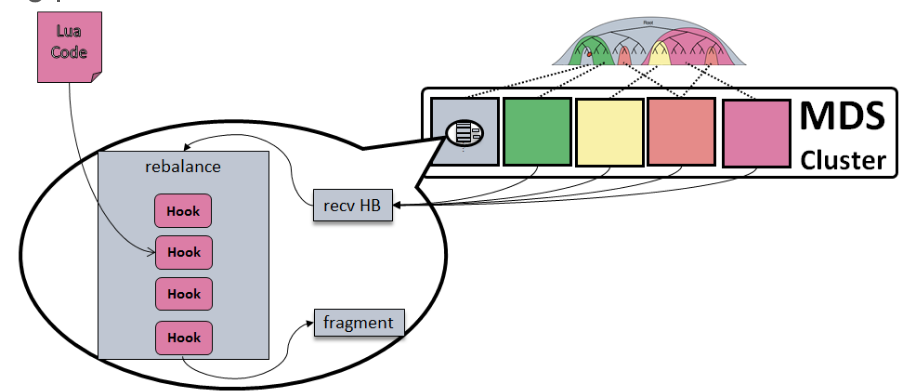
\includegraphics[width=19pc,angle=0]{figures/arch-mantle.png}\\
%  \caption{The Mantle API lets adminstrators control load balancing by
%  changing the poicies for how to distribution or concentrate file system
%  metadata. It was merged into CephFS and inherits many aspects of that
%  architecture. Although it has the load balancing structure and logic from
%  CephFS (gray boxes), the actual API is not dependent on that code base.}
%  \label{fig:arch-mantle}
%\end{figure}
%\begin{figure}[tb]
%  \noindent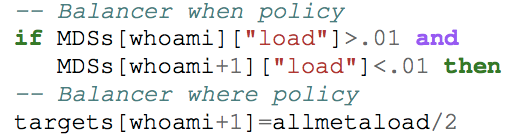
\includegraphics[width=19pc,angle=0]{figures/arch-mantle-example.png}\\
%  \caption{The Greedy Spill balancer written in Lua using the Mantle API.}
%  \label{fig:arch-mantle-example}
%\end{figure}
%

\subsubsection*{Results}

The right most graph of Figure~\ref{fig:methodology-tradeoff} shows the results
of using the Mantle API to program a dynamic load balancing policy with two
phases into ParSplice:

\begin{itemize}
  \item unlimited growth: cache increases on every write
  \item \(n\) key limit: cache maintained at this size
\end{itemize}

We trigger the policy switch at 100K keys to absorb the flash crowd at the
beginning of the run. Once triggered, keys are evicted to bring the size of the
cache down to the threshold and the least recently keys are actively evicted.
In that bar chart, the cache sizes are along the \(x\)-axis.

% results: same level of performance can be achived 
The dynamic policies show better performance than the single \(n\) key
policies. The performance and memory utilization for 100K is the same as the
100K bar in the middle graphs but the rest reduce the size of the keyspace
after the read flash crowd. This reduced read/write traffic on the
persistent database and lowers the number of stalls.  The worst performing
policy is the 10 key cache, which achieves 94\% of the performance while only
using 40KB of memory. 

% caveats: it is calculating 90% of the trajectory, memory value reported is final
\subsubsection*{Caveats}

The results from the right most graph in Figure~\ref{fig:methodology-tradeoff}
are slightly deceiving for three reason: (1) segments take longer to generate
later in the run, (2) the memory footprint is the value at the end of 2.5
hours, and (3) this policy only works well for the 2.5 hour run.  For (1), the
curving down of the simulation vs. wall-clock time is shown in
Figure~\ref{fig:methodology-trajectory}; as the nanoparticle grows it takes
longer to generate segments so by the time we reach 2 hours, over 90\% of the
trajectory is already generated.  For (2), the memory footprint is around 0.4GB
until we reach 100K key threshold. In Figure~\ref{fig:methodology-tradeoff} we plot the
final value. For (3), Figure~\ref{fig:methodology-trajectory} shows that the
cache fills up with 100K keys at time 7200 seconds and its size is reduced to the size
listed in the legend.  The curves stay close to ``Unlimited" for up to an hour
after the cache is reduced but eventually flatten out as the persistent
database gets overloaded. 10K and 100K follow the ``Unlimited" curve the
longest and are sufficient policies for the 2.5 hour runs but anything longer
would need a different dynamic load balancing policy.

\begin{figure}[tbh]
  \noindent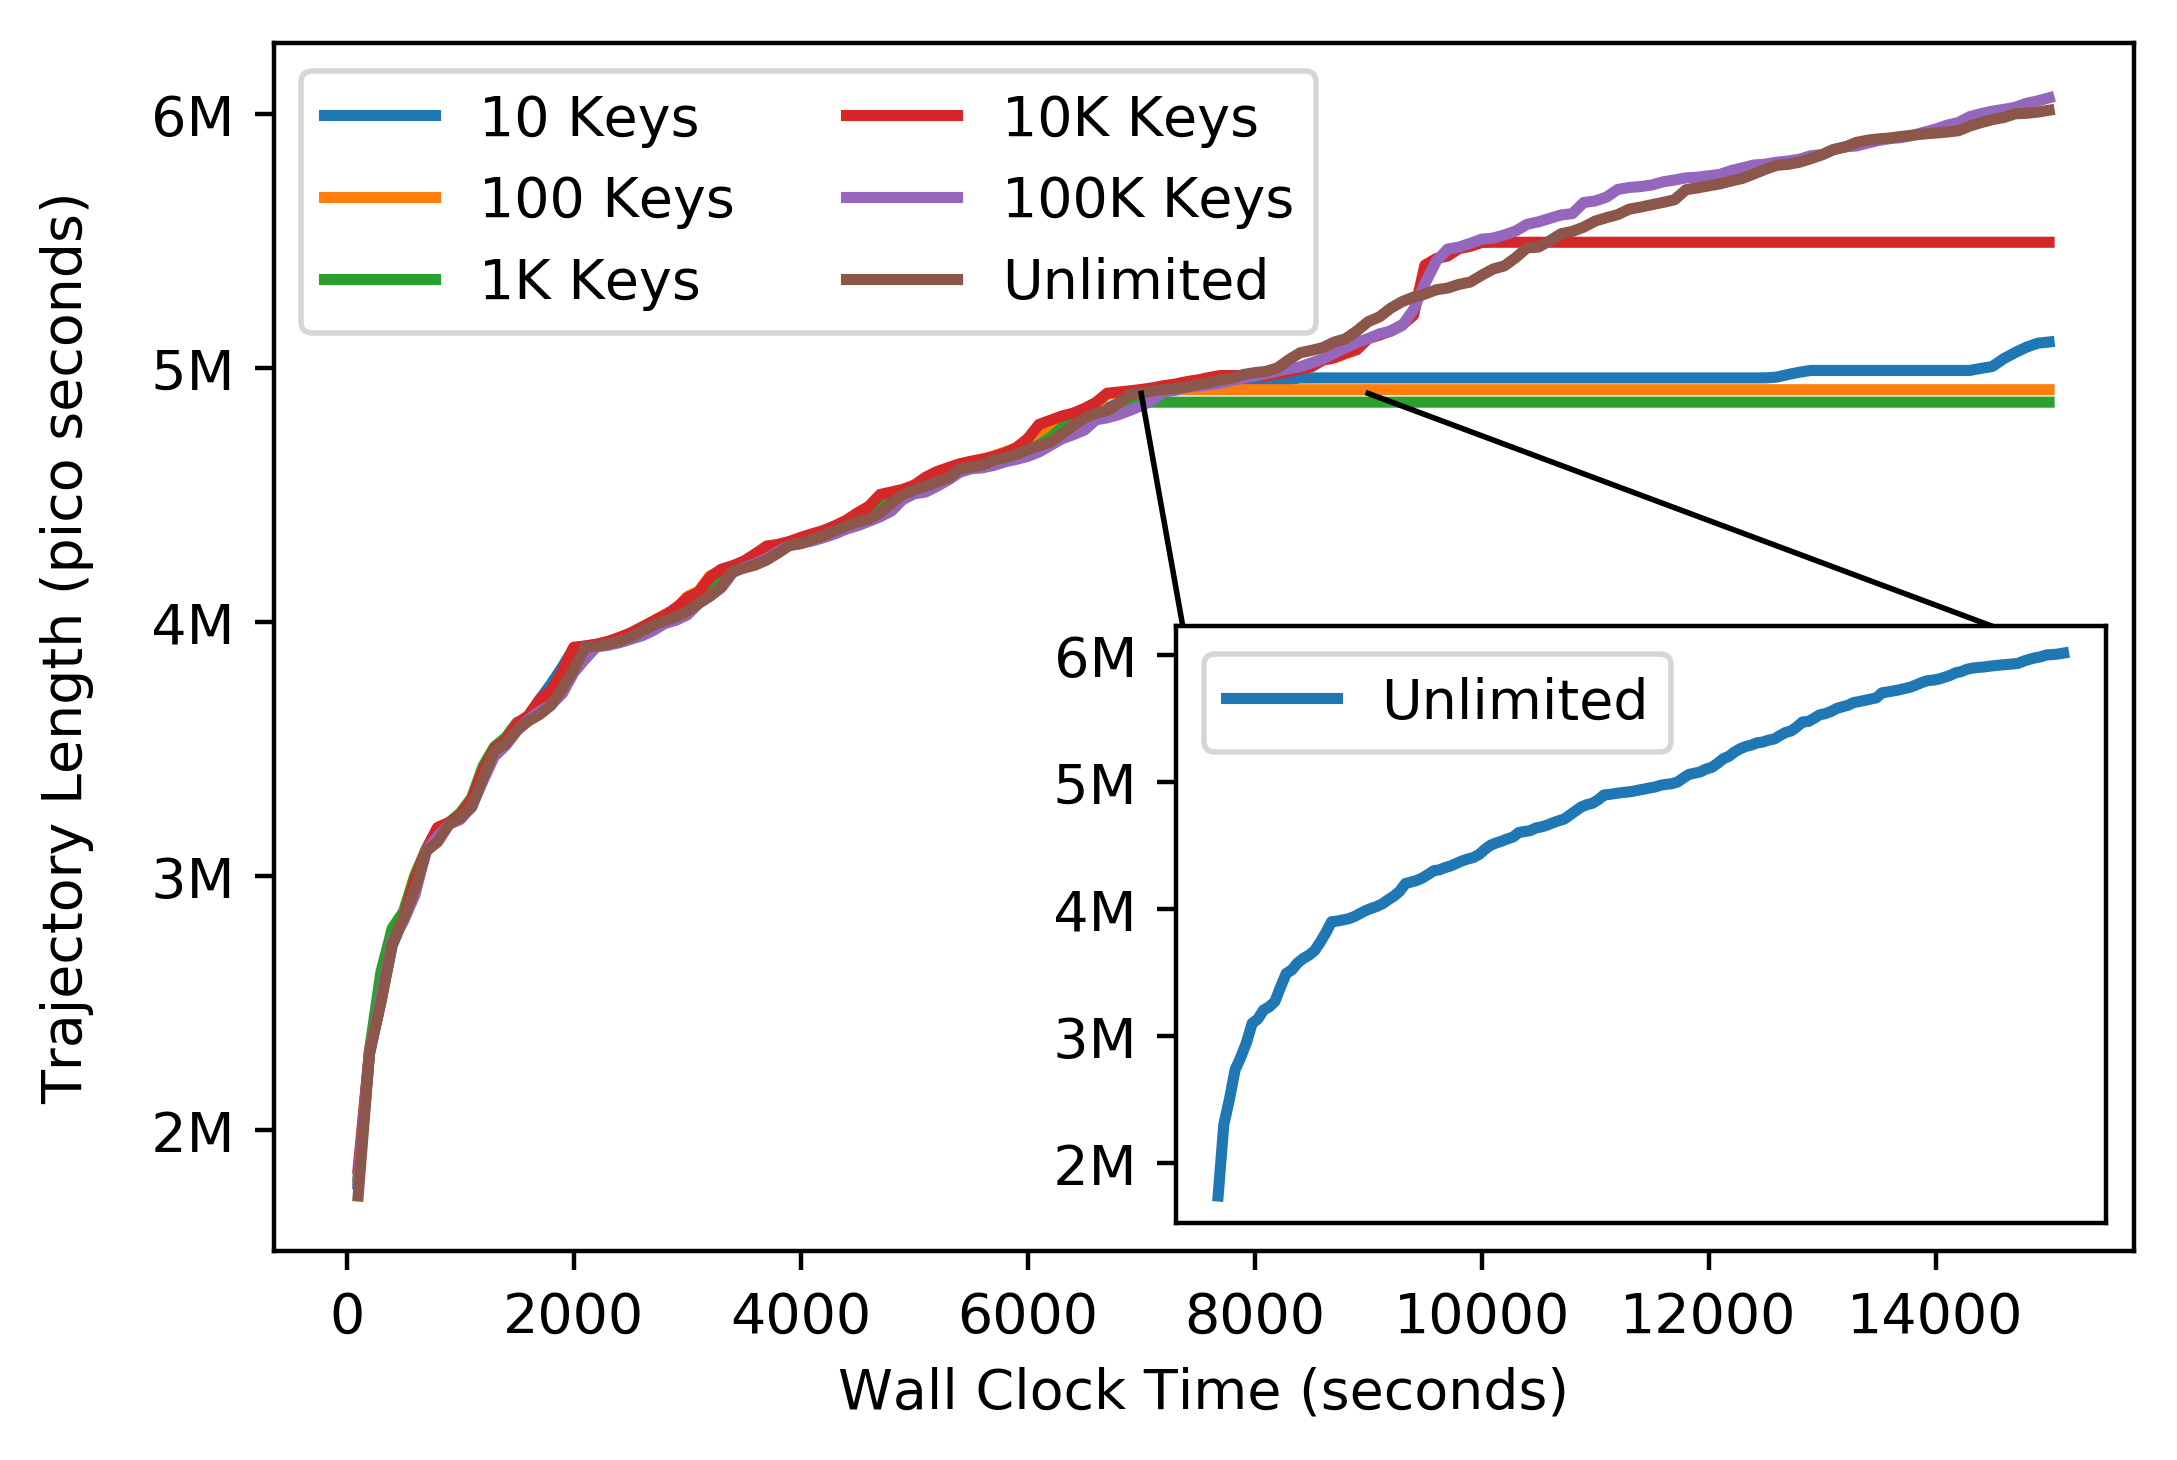
\includegraphics[width=0.45\textwidth]{figures/methodology-trajectory.png}\\
  \caption{The rate that the trajectory is computed decays over time (which is
  expected) but this skews the performance improvements in
  Figure~\ref{fig:methodology-tradeoff}. While the dynamic policy we designed
  does not work for 4 hours, it does work for our target
  runtime of 2.5 hours. \label{fig:methodology-trajectory}}
\end{figure}

% wht the result is still valie
Despite these caveats, the result is still valid: we found a dynamic load
balancing policy that absorbs the cost of a high read throughput on a small
keyspace and reduces the memory pressure for a 2.5 hour run. Our experiments
show the effectiveness of the load balancing policy engine we integrated into
ParSplice, not that we were able to identify the best policy for all system
setups ({\it i.e.} different ParSplice parameters, number of worker nodes, and
job lengths).  To solve that problem, we need a way to identify what thresholds
we should use for different job permutations.

\section{Using ML for the Keyspace}

We proved in the previous section that an optimial policy, based on the read
burstiness at the beginning of the run,  exists for a 100K growth rate on 8
nodes, but we cannot re-do this analysis for every workload, system, and
parameter permutation.  Fortunately, Section~\S\ref{sec:results} shows that the
keyspace size and activity is structured. so rather than finding policies hand
again for every cluster size, growth rate, and temperature, in this section we
use machine learning to inform the Mantle policy engine.

% implementation: 
We feed the read request rate from the 100K and 1M runs in
Figure~\ref{fig:motivation-regimes} into the K-means clustering algorithm as
(timestamp, ops/second) tuples. We weight the timestamp and ops/second equally
and set the number of clusters to be 4. We chose this initial K  based on
visual inspection of Figure~\ref{fig:motivation-regimes}, where it appears that
there are 4 workload phases: one plateau of redundant reads at the beginning,
decreasing requests per second, and then two plateaus of steady requests per
second. Knowing that the setup parameters transform the request rates
temporally or spatially, this same initial K should work for all setups. Once
the algorithm identifies the workload regimes, we select the start of the third
regime as the point to switch to a fixed sized cache because the request rate has
lowered to sustainable levels for the persistent database.

\subsubsection*{Results}

We plot throughput over time in Figure~\ref{figures/futurework-regimes.png} and
color each point with its assigned group. The black squares are the centroids,
also known as the center of K-means groups.  We run the algorithm for a variety
of request rate traces but only show the setups from
Figure~\ref{fig:motivation-regimes}. We also annotate the graphs with the
suggested cache size, which is calculated by looking up the timestamp for the
third regime that corresponds to the keyspace size in our performance counters.

% results: 1. ideentifies 4 phases, 2. picks different timestamps for the third
% regime, suggests proper key values.
The algorithm properly identifies the 4 workload phases: the plateau of
redundant reads, the phase with a large decrease in request rate, and the two
plateaus of steady read requests. It also picks different timestamps for the
start of the third regime, which aligns with our keyspace analysis and our
assertion that the growth parameters affect how long it takes the workload to
reach a certain phase.  Finally, the algorithm picks reasonable values for the
key cache size. The 100K growth rate selects a 55K cache size, which is between
our benchmarked optimal threshold for the high watermark value chosen to
absorb the read burst (100K) and the lower cache size we limit the system to
after the initial burst (10K). This result both reaffirms the results from the
previous section and provides hope that we can avoid lengthy paramaters sweeps
for ParSplice in the future.

\begin{figure}[tbh]
\noindent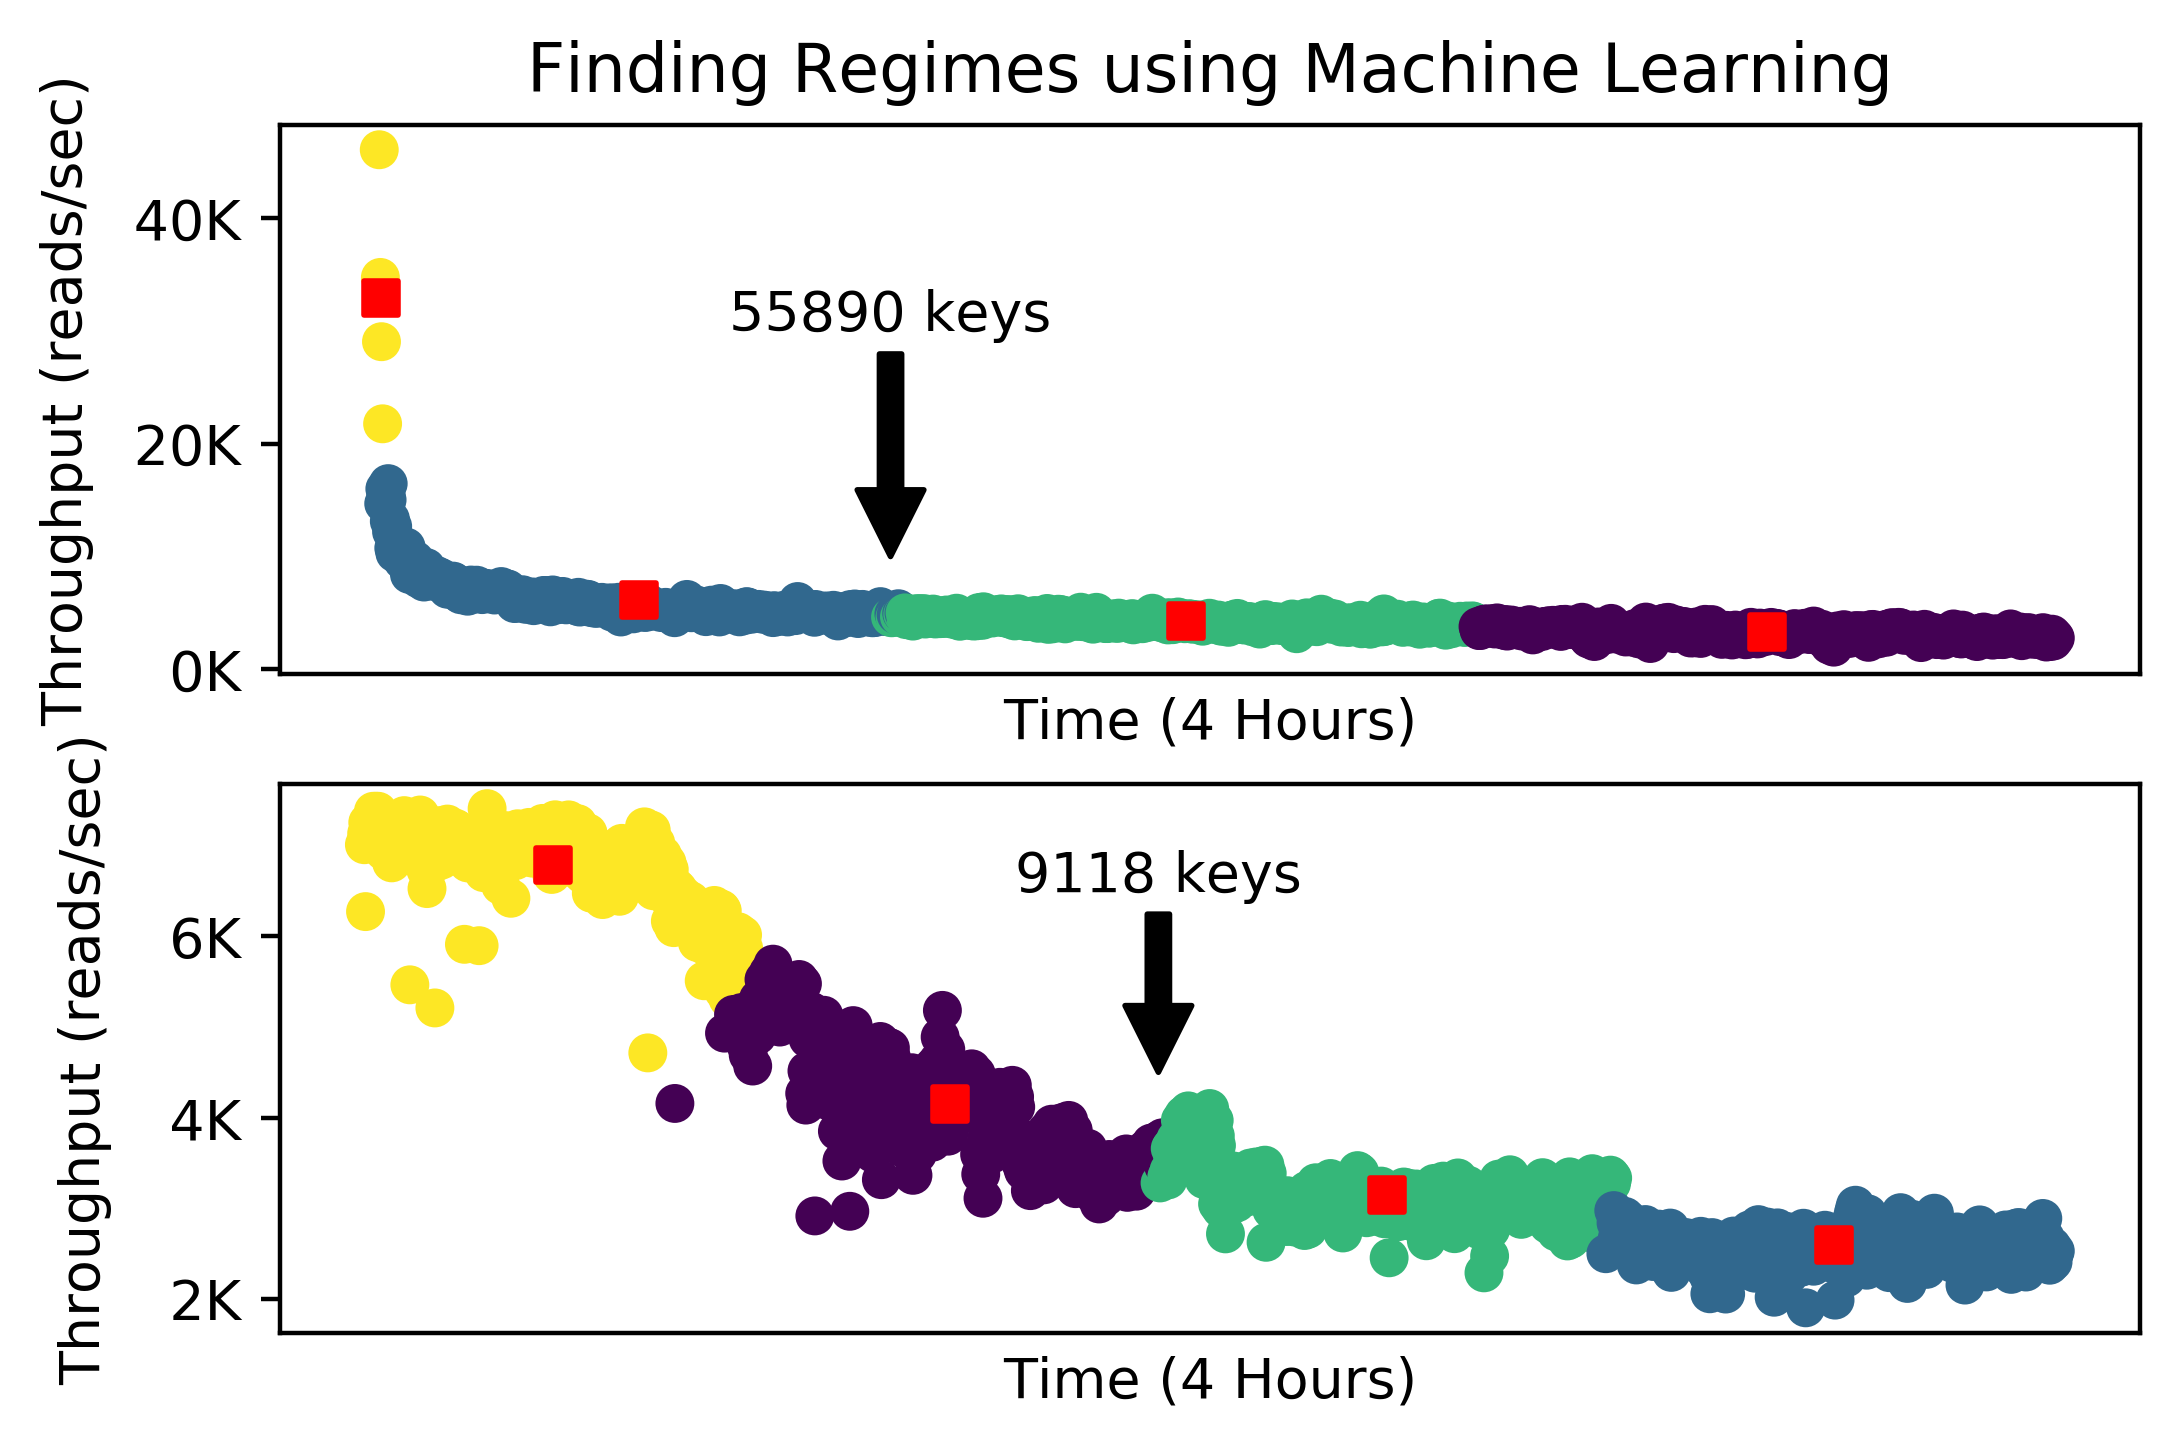
\includegraphics[width=0.45\textwidth]{figures/futurework-regimes.png}\\
  \caption{Learning the workload regimes with K-Means clustering helps pick
  keyspace size thresholds that can be fed into a dynamic load balancing policy
  engine, like Mantle. Specifying 4 clusters and selecting the third for
  informing the policy switch returns keyspace size thresholds similar to the
  values we found by hand in
  Section~\S\ref{sec:the-need-for-dynamic-load-balancing-policies}.
\label{fig:futurework-regimes}}
\end{figure}
